% IEEE conference version (IEEE Conference Template v1.0, 2026/10/15). Build: ./build.sh
% Modes: add [doubleanonymous] or [singleanonymous] for review (adds line numbers); default is camera-ready.
% Requires the official ieeeconf.cls v1.0. The ieeeconf.cls in this folder is a preview stand-in (see its header).
\documentclass[9pt]{ieeeconf}

%% Packages (from the template, then the ones this paper needs).
\usepackage{bm}
\usepackage{etoolbox}
\usepackage{siunitx}
\robustify\bfseries
\usepackage{booktabs}
\usepackage{enumitem}
\usepackage{tikz}
\usetikzlibrary{arrows.meta,calc,decorations.pathreplacing}
\usepackage[capitalize,nameinlink]{cleveref}
\crefname{equation}{}{}
\Crefname{equation}{Equation}{Equations}
\crefname{appendix}{Appendix}{Appendices}
\Crefname{appendix}{Appendix}{Appendices}

\graphicspath{{figures/}}

%% Paper terms. Use these macros so a rename is one edit.
\newcommand{\ST}{Soft Thinking}
\newcommand{\GST}{Gumbel Soft Thinking}
\newcommand{\ctrl}{random-residual control}

\title{Superposition or Sampling in Disguise?\\What Soft Thinking Stores, Feeds and Uses}

\addauthor{Hassan Nafees}{1}
\addaffiliation{1}{Department of Computer Science, FAST National University of Computer and Emerging Sciences, Karachi, Pakistan\\\texttt{k230769@nu.edu.pk}}

\begin{document}

\maketitle

\begin{abstract}
\ST{} feeds a reasoning model blends of token embeddings instead of single tokens, in the hope that the model can
carry several candidate continuations in superposition.
Recent work adds Gumbel noise to the blend weights to avoid greedy collapse.
With that noise, the top token of each blend is distributed exactly as a sampled token, so \GST{} is ordinary sampling
plus a residual weight on the other candidates.
We test superposition at the level of single tokens in DeepSeek-R1-Distill-Qwen-1.5B on GSM8K: does the residual % SETUP
survive the layers, persist in the cache, and change what the model does?
Exact 50/50 blends of two candidates, a forced superposition built at the input,
collapse gradually through the layers.
Information about the runner-up persists in the keys and values of layers 0 to 7 and shifts the projected % C21.10
next-token readout of later text toward it ($+0.44$, 95\% CI [0.35, 0.53], number vs number forks); % C21.7-8
on the model's own path the shift is not detectable.
In real runs the residual is small (median 0.12 at forks), and the top token changes as often as under % C22.12
sampling (0.45 vs 0.45). % C22.4
A coupled ablation with shared noise shows that the model reads the residual: it moves next-token predictions a
median 3.9 times as much as a random residual of the same size (95\% CI [3.1, 5.0]). % C23.15
Accuracy does not change detectably (88 vs 86 of 100; paired difference $+2$ points, 95\% CI [$-5$, $+9$]), % C23.1 C23.17
and the real and random residuals change sampling's final answer on largely the same problems % C23.18
(10 shared, 6 for each alone). % C23.18
Token-level superposition is therefore present in the input and read by the model, but we detect no use of it in
the answers of this model; whether whole reasoning paths are carried in superposition is not tested here.
The main predictions were committed before the runs, and every number from our experiments is recomputed from saved
outputs.
\end{abstract}

\section{Introduction}\label{sec:intro}

A reasoning model that writes out its chain of thought commits to one token at every step \cite{wei2022chain}.
The other candidates at that step are discarded.
Latent reasoning methods relax this commitment by feeding the model continuous states instead of tokens
\cite{hao2024coconut,zhang2025soft}.
A common motivation is \emph{superposition}: a continuous state might hold several candidate paths at once and let
the model explore them in parallel.
In theory this can help, since a two-layer transformer with continuous thoughts can solve graph reachability by
keeping several search frontiers in one state \cite{zhu2025superposition}.
\ST{} \cite{zhang2025soft} was proposed with the same intuition.
It needs no training: at each thinking step it feeds the probability-weighted average of the top candidates'
embeddings in place of one sampled token.

Whether off-the-shelf models use these blends is contested.
Wu et al.~\cite{wu2025single} find that vanilla \ST{} is dominated by its top token and drifts into greedy, repetitive
decoding, which they call the Greedy Pitfall.
They add Dirichlet or Gumbel noise to the blend weights and report small accuracy gains over matched sampling.
Rizvi-Martel et al.~\cite{rizvimartel2026illusion} find no sign that vanilla \ST{} reasons in superposition,
and Backour~\cite{backour2026dynamics} shows that pretrained models collapse injected mixtures of embeddings through depth.

Gumbel noise also changes what the superposition question asks.
By the Gumbel-max trick \cite{gumbel1954statistical,maddison2014sampling}, the top token of a Gumbel blend is
distributed exactly as a sampled token.
\GST{} therefore feeds the token that sampling would feed, plus a \emph{residual}: the blend weight that sits on the
other candidates (\cref{fig:concept}).
If the model ignores the residual, \GST{} is sampling in disguise.
If the model carries both candidates forward and uses them, it reasons in genuine superposition.
A third outcome lies between the two: the model may read the residual without its answers depending on it.
Our research question is which of these holds:
\begin{quote}
\emph{Does \GST{} reason in superposition, or is it sampling in disguise?}
\end{quote}
We answer it at the level of single tokens.
Every blend in this paper, whether an exact 50/50 blend or one fed by \GST{}, is a \emph{forced} superposition,
built at the input, as opposed to a \emph{learned} one that emerges from training \cite{rizvimartel2026illusion}.
We ask whether one token position carries two candidates and whether that changes what the model does.
Whether whole reasoning paths are carried in superposition over many steps, as in the graph-search construction of
Zhu et al.~\cite{zhu2025superposition}, is a different question that we do not test.

We split the question into four measurements (\cref{fig:questions}) on DeepSeek-R1-Distill-Qwen-1.5B % SETUP
\cite{deepseekai2025r1,guo2025nature} solving GSM8K problems \cite{cobbe2021gsm8k}.
Q1 asks whether a blend of two candidates survives the layers.
Q2 asks whether information about the losing candidate, the runner-up, persists in the key-value cache and shifts
what later text predicts.
Q3 asks what blends the noise actually feeds in real runs.
Q4 asks whether the residual changes the model's next-token predictions and its final answers.
We committed numeric predictions for the main tests before running them.

Our evidence supports three statements about token-level superposition in this model.
First, the top token of \GST{} is a sampled token.
Second, the residual is read: it shifts the model's next-token predictions far more than a random residual of the
same size.
Third, no change in accuracy is detected on 100 problems, with a paired interval that still allows a few points % C23.1
either way.
The superposition is present in the input and read, but we find no evidence that it is used.
Our contributions are as follows.
\begin{itemize}[leftmargin=1.2em,itemsep=2pt,topsep=3pt]
\item \textbf{\GST{} is sampling plus a residual.}
We make the Gumbel-max consequence explicit and confirm it in logged runs:
at forks the top token changes at a rate of 0.45, the same as under sampling (0.45). % C22.4
Real forks feed lopsided blends, near one token at 47\% of forks, with a median residual of 0.12. % C22.11 C22.12
Dirichlet noise does not even match sampling: its top token leans toward the model's first choice
(\cref{sec:q3}).
\item \textbf{The runner-up persists in the cache.}
Blends collapse gradually through the layers, as Backour~\cite{backour2026dynamics} found in other models.
Yet information about the runner-up persists, mostly in the keys and values of layers 0 to 7, which close a pooled % C21.10
share of 0.71 to 0.91 of the readback gap (pre-registered); part of this is an echo of the input in the first layers. % C21.10
Later text that turns toward the runner-up shifts the projected next-token readout toward it ($+0.44$ for number % C21.7-8
vs number forks).
On the model's own path the shift is not detectable (\cref{sec:q1,sec:q2}).
\item \textbf{The model reads the residual, but accuracy does not change detectably.}
A coupled ablation runs sampling, \ST{} and a \ctrl{} in lockstep with shared noise.
\ST{} leaves sampling first on 59 problems against 24 for the control ($p = 0.0002$) % C23.5-6
and moves next-token predictions a median 3.9 times as much (95\% CI [3.1, 5.0]). % C23.15
Accuracy does not change detectably (88 vs 86 of 100; paired difference $+2$ points, 95\% CI [$-5$, $+9$]), % C23.1 C23.17
and paired by problem, the real and random residuals change sampling's final answer on mostly the same problems
(\cref{sec:q4}).
\item \textbf{A checkable study.}
Predictions were committed before the runs and the failed ones are reported as written (\cref{app:prereg}).
Every number from our experiments is recomputed from saved outputs by scripts in our repository (\cref{app:repro}).
\end{itemize}

\begin{figure*}[t]
\centering
% Fig 1: concept diagram (TikZ). In the paper:
%   \begin{figure*}[t] \centering % Fig 1: concept diagram (TikZ). In the paper:
%   \begin{figure*}[t] \centering \input{figures/fig1.tex} \caption{...} \label{fig:concept} \end{figure*}
% Preamble needs \usepackage{tikz} and \usetikzlibrary{arrows.meta,decorations.pathreplacing}.
% Drawn at final size (under the 6.5 in text width); include it as is, never scaled, so text stays 7-8 pt.
% Draft caption:
%   Gumbel Soft Thinking feeds the sampled token plus a residual. At each thinking step the model gives next-token
%   probabilities. Sampling feeds one token. Gumbel Soft Thinking adds Gumbel noise and feeds the softmax-weighted
%   mix of token embeddings; by the Gumbel-max trick, its top token is distributed exactly as the sampled one (and
%   is the same token when both use the same noise, as in Exp 23), so all it adds is the residual (blue). The
%   random-residual control keeps the top token and the residual's size but moves the residual to a random token
%   (orange). Weights are illustrative.
% No data numbers. Colours match figures/style.py: sampling grey, Gumbel Soft Thinking blue, control orange.
\definecolor{fsamp}{HTML}{7F7F7F}%
\definecolor{fsoft}{HTML}{0072B2}%
\definecolor{frand}{HTML}{E69F00}%
\definecolor{fdark}{HTML}{333333}%
\begin{tikzpicture}[x=1cm, y=1cm, font=\footnotesize, line width=0.5pt,
    >={Stealth[length=4.5pt, width=4pt]},
    wire/.style={line width=0.8pt, fdark},
    lab/.style={font=\scriptsize, inner sep=1pt, text=fdark},
    inbar/.style={font=\scriptsize\ttfamily, text=white, inner sep=0pt},
    brace/.style={decorate, decoration={brace, amplitude=3.5pt}, black!55, line width=0.5pt}]
\def\L{5.5}            % bar length = weight 1
\def\xb{7.45}           % bar start
\pgfmathsetmacro{\xt}{\xb + 0.75*\L}   % end of the top token (weight 0.75)
\pgfmathsetmacro{\xe}{\xb + \L}

% ---- next-token probabilities ----
\node[lab, align=center, anchor=south] at (1.45, 2.95) {next-token\\[-1pt]probabilities};
\foreach \x/\p/\t in {0.8/0.55/7, 1.45/0.35/8, 2.1/0.10/12} {
  \draw[fdark, fill=white] (\x-0.21, 0.6) rectangle (\x+0.21, 0.6+3.9*\p*0.95);
  \node[lab, font=\scriptsize\ttfamily, anchor=north] at (\x, 0.55) {\t};
}
\draw[fdark] (0.4, 0.6) -- (2.5, 0.6);

% ---- three ways to feed it ----
\draw[wire] (2.65, 1.975) -- (3.2, 1.975);
\draw[wire] (3.2, 0.725) -- (3.2, 3.225);
\foreach \y/\t in {3.225/{sample one token}, 1.975/{add Gumbel noise, softmax}, 0.725/{same, then move the residual}} {
  \draw[wire, ->] (3.2, \y) -- (\xb-0.08, \y);
  \node[lab, anchor=south] at ({(3.2+\xb)/2}, \y+0.03) {\t};
}
\fill[fdark] (3.2, 1.975) circle (1.3pt);

% ---- what is fed: one bar per method, length = total weight 1 ----
\fill[fsamp] (\xb, 3.0) rectangle (\xe, 3.45);
\node[inbar] at ({(\xb+\xt)/2}, 3.225) {7};
\fill[fsamp] (\xb, 1.75) rectangle (\xt, 2.2);
\fill[fsoft] (\xt, 1.75) rectangle ({\xb+0.95*\L}, 2.2);
\fill[fsoft!55] ({\xb+0.95*\L}, 1.75) rectangle (\xe, 2.2);
\draw[white, line width=0.8pt] ({\xb+0.95*\L}, 1.75) -- ({\xb+0.95*\L}, 2.2);
\node[inbar] at ({(\xb+\xt)/2}, 1.975) {7};
\node[inbar] at ({\xt+0.1*\L}, 1.975) {8};
\fill[fsamp] (\xb, 0.5) rectangle (\xt, 0.95);
\fill[frand] (\xt, 0.5) rectangle (\xe, 0.95);
\node[inbar] at ({(\xb+\xt)/2}, 0.725) {7};
\draw[black!35, dash pattern=on 2pt off 1.5pt] (\xt, 0.35) -- (\xt, 3.6);

% ---- braces: the shared top token and the residual ----
\draw[brace] (\xb, 3.62) -- (\xt-0.04, 3.62) node[midway, above=4pt, lab] {top token (the same in all three)};
\draw[brace] (\xt+0.04, 3.62) -- (\xe, 3.62) node[midway, above=4pt, lab] {residual};

% ---- names ----
\foreach \y/\c/\n/\d in {3.225/fsamp/{sampling}/{one token}, 1.975/fsoft/{Gumbel Soft Thinking}/{token $+$ residual},
                         0.725/frand/{random-residual control}/{residual on a random token}} {
  \node[lab, anchor=west, align=left, text=\c] at (\xe+0.18, \y) {\textbf{\n}\\[-1pt]\textcolor{fdark}{\d}};
}
\end{tikzpicture}
 \caption{...} \label{fig:concept} \end{figure*}
% Preamble needs \usepackage{tikz} and \usetikzlibrary{arrows.meta,decorations.pathreplacing}.
% Drawn at final size (under the 6.5 in text width); include it as is, never scaled, so text stays 7-8 pt.
% Draft caption:
%   Gumbel Soft Thinking feeds the sampled token plus a residual. At each thinking step the model gives next-token
%   probabilities. Sampling feeds one token. Gumbel Soft Thinking adds Gumbel noise and feeds the softmax-weighted
%   mix of token embeddings; by the Gumbel-max trick, its top token is distributed exactly as the sampled one (and
%   is the same token when both use the same noise, as in Exp 23), so all it adds is the residual (blue). The
%   random-residual control keeps the top token and the residual's size but moves the residual to a random token
%   (orange). Weights are illustrative.
% No data numbers. Colours match figures/style.py: sampling grey, Gumbel Soft Thinking blue, control orange.
\definecolor{fsamp}{HTML}{7F7F7F}%
\definecolor{fsoft}{HTML}{0072B2}%
\definecolor{frand}{HTML}{E69F00}%
\definecolor{fdark}{HTML}{333333}%
\begin{tikzpicture}[x=1cm, y=1cm, font=\footnotesize, line width=0.5pt,
    >={Stealth[length=4.5pt, width=4pt]},
    wire/.style={line width=0.8pt, fdark},
    lab/.style={font=\scriptsize, inner sep=1pt, text=fdark},
    inbar/.style={font=\scriptsize\ttfamily, text=white, inner sep=0pt},
    brace/.style={decorate, decoration={brace, amplitude=3.5pt}, black!55, line width=0.5pt}]
\def\L{5.5}            % bar length = weight 1
\def\xb{7.45}           % bar start
\pgfmathsetmacro{\xt}{\xb + 0.75*\L}   % end of the top token (weight 0.75)
\pgfmathsetmacro{\xe}{\xb + \L}

% ---- next-token probabilities ----
\node[lab, align=center, anchor=south] at (1.45, 2.95) {next-token\\[-1pt]probabilities};
\foreach \x/\p/\t in {0.8/0.55/7, 1.45/0.35/8, 2.1/0.10/12} {
  \draw[fdark, fill=white] (\x-0.21, 0.6) rectangle (\x+0.21, 0.6+3.9*\p*0.95);
  \node[lab, font=\scriptsize\ttfamily, anchor=north] at (\x, 0.55) {\t};
}
\draw[fdark] (0.4, 0.6) -- (2.5, 0.6);

% ---- three ways to feed it ----
\draw[wire] (2.65, 1.975) -- (3.2, 1.975);
\draw[wire] (3.2, 0.725) -- (3.2, 3.225);
\foreach \y/\t in {3.225/{sample one token}, 1.975/{add Gumbel noise, softmax}, 0.725/{same, then move the residual}} {
  \draw[wire, ->] (3.2, \y) -- (\xb-0.08, \y);
  \node[lab, anchor=south] at ({(3.2+\xb)/2}, \y+0.03) {\t};
}
\fill[fdark] (3.2, 1.975) circle (1.3pt);

% ---- what is fed: one bar per method, length = total weight 1 ----
\fill[fsamp] (\xb, 3.0) rectangle (\xe, 3.45);
\node[inbar] at ({(\xb+\xt)/2}, 3.225) {7};
\fill[fsamp] (\xb, 1.75) rectangle (\xt, 2.2);
\fill[fsoft] (\xt, 1.75) rectangle ({\xb+0.95*\L}, 2.2);
\fill[fsoft!55] ({\xb+0.95*\L}, 1.75) rectangle (\xe, 2.2);
\draw[white, line width=0.8pt] ({\xb+0.95*\L}, 1.75) -- ({\xb+0.95*\L}, 2.2);
\node[inbar] at ({(\xb+\xt)/2}, 1.975) {7};
\node[inbar] at ({\xt+0.1*\L}, 1.975) {8};
\fill[fsamp] (\xb, 0.5) rectangle (\xt, 0.95);
\fill[frand] (\xt, 0.5) rectangle (\xe, 0.95);
\node[inbar] at ({(\xb+\xt)/2}, 0.725) {7};
\draw[black!35, dash pattern=on 2pt off 1.5pt] (\xt, 0.35) -- (\xt, 3.6);

% ---- braces: the shared top token and the residual ----
\draw[brace] (\xb, 3.62) -- (\xt-0.04, 3.62) node[midway, above=4pt, lab] {top token (the same in all three)};
\draw[brace] (\xt+0.04, 3.62) -- (\xe, 3.62) node[midway, above=4pt, lab] {residual};

% ---- names ----
\foreach \y/\c/\n/\d in {3.225/fsamp/{sampling}/{one token}, 1.975/fsoft/{Gumbel Soft Thinking}/{token $+$ residual},
                         0.725/frand/{random-residual control}/{residual on a random token}} {
  \node[lab, anchor=west, align=left, text=\c] at (\xe+0.18, \y) {\textbf{\n}\\[-1pt]\textcolor{fdark}{\d}};
}
\end{tikzpicture}

\caption{\GST{} feeds the sampled token plus a residual.
At each thinking step the model gives next-token probabilities.
Sampling feeds one token.
\GST{} adds Gumbel noise and feeds the softmax-weighted mix of token embeddings.
By the Gumbel-max trick, its top token is distributed exactly as the sampled one,
and it is the same token when both use the same noise in the same context, as in our coupled ablation (\cref{sec:q4}).
So all it adds is the residual (blue).
The \ctrl{} keeps the top token and the residual's size but moves the residual to a random token (orange).
Weights are illustrative.}
\label{fig:concept}
\end{figure*}

\begin{figure*}[t]
\centering
% Fig 2: the four questions (TikZ). Follows Fig 1 (the concept). In the paper:
%   \begin{figure*}[t] \centering % Fig 2: the four questions (TikZ). Follows Fig 1 (the concept). In the paper:
%   \begin{figure*}[t] \centering \input{figures/fig2.tex} \caption{...} \label{fig:questions} \end{figure*}
% Preamble needs \usepackage{tikz} and \usetikzlibrary{arrows.meta}. Drawn at final size; include it as is.
% Draft caption:
%   The four questions we test. (1) Does a blend of two candidates survive the layers, or snap to one of them
%   (Fig. 3)? (2) Is the runner-up stored in the K,V cache, and can later steps read it back (Figs. 4-5)?
%   (3) What blends does the noise actually feed in real runs (Fig. 6)? (4) Does the residual move the model's
%   next-token predictions more than a random residual of the same size (Fig. 7, Table 1)? Drawings are schematic.
% No data numbers: every position and bar is illustrative.
% Colours match figures/style.py: sampling grey, Gumbel Soft Thinking blue, random-residual control orange.
\definecolor{fsamp}{HTML}{7F7F7F}%
\definecolor{fsoft}{HTML}{0072B2}%
\definecolor{frand}{HTML}{E69F00}%
\definecolor{fdark}{HTML}{333333}%
\definecolor{fcell}{HTML}{E9E9EC}%
\begin{tikzpicture}[x=1cm, y=1cm, font=\footnotesize, line width=0.5pt,
    >={Stealth[length=4pt, width=3.5pt]},
    lab/.style={font=\scriptsize, inner sep=1pt, text=black!60},
    qm/.style={circle, fill=fdark, text=white, font=\scriptsize\bfseries, inner sep=0pt, minimum size=10.5pt},
    qt/.style={anchor=north west, font=\footnotesize\bfseries, text=fdark, inner sep=0pt, text width=3.4cm,
               align=left, execute at begin node={\hyphenpenalty=10000}}]

\foreach \x in {4.075, 8.225, 12.375} \draw[black!15] (\x, 0.05) -- (\x, 3.65);

% ---------- 1: does the blend survive the layers? ----------
\begin{scope}[shift={(0, 0)}]
  \node[qm] at (0.17, 3.5) {1}; \node[qt] at (0.42, 3.6) {Does the blend survive the layers?};
  \foreach \y/\f in {0.6/0.5, 1.45/0.72, 2.3/0.87} {
    \draw[black!30, line width=0.8pt] (1.0, \y) -- (3.6, \y);
    \draw[fdark, fill=white] (1.0, \y) circle (0.075);
    \fill[fsamp] (3.6, \y) circle (0.075);
    \fill[fsoft] (1.0+2.6*\f, \y) circle (0.095);
  }
  \draw[->, fsoft!60, dash pattern=on 1.5pt off 1.2pt] (2.38, 0.72) .. controls (2.52, 1.05) .. (2.79, 1.34);
  \draw[->, fsoft!60, dash pattern=on 1.5pt off 1.2pt] (2.95, 1.57) .. controls (3.08, 1.9) .. (3.22, 2.18);
  \node[lab, anchor=east] at (0.85, 0.6) {input};
  \node[lab, anchor=east] at (0.85, 2.3) {output};
  \node[lab, font=\scriptsize\ttfamily, text=fdark] at (1.0, 0.3) {8};
  \node[lab, font=\scriptsize\ttfamily, text=fdark] at (3.6, 0.3) {7};
  \node[lab, text=fsoft] at (2.3, 0.3) {blend};
\end{scope}

% ---------- 2: is the runner-up stored? ----------
\begin{scope}[shift={(4.15, 0)}]
  \node[qm] at (0.17, 3.5) {2}; \node[qt] at (0.42, 3.6) {Does the runner-up persist?};
  \foreach \i in {0,...,4} \foreach \j in {0,...,3}
    \fill[fcell] (0.75+0.57*\i, 0.5+0.45*\j) rectangle (1.25+0.57*\i, 0.88+0.45*\j);
  \fill[fsoft] (1.32, 0.5) rectangle (1.82, 0.88);
  \fill[fsoft!60] (1.32, 0.95) rectangle (1.82, 1.33);
  \fill[fsoft!22] (1.32, 1.4) rectangle (1.82, 1.78);
  \draw[->, fdark, line width=0.7pt] (3.28, 2.3) .. controls (3.15, 2.85) and (1.75, 2.85) .. (1.6, 2.32);
  \node[lab, text=fdark] at (2.44, 2.92) {read later};
  \draw[->, black!45] (0.5, 0.5) -- (0.5, 2.23) node[midway, lab, rotate=90, anchor=south] {layers};
  \node[lab, text=fsoft] at (1.57, 0.27) {fork};
  \draw[->, black!45] (2.1, 0.27) -- (3.0, 0.27);
  \node[lab, anchor=west] at (3.03, 0.27) {steps};
\end{scope}

% ---------- 3: what does the noise feed? ----------
\begin{scope}[shift={(8.3, 0)}]
  \node[qm] at (0.17, 3.5) {3}; \node[qt] at (0.42, 3.6) {What does the noise feed?};
  \foreach \r [count=\k] in {0.04, 0.15, 0.02, 0.38, 0.07, 0.01, 0.26, 0.05} {
    \pgfmathsetmacro{\yy}{2.55-0.27*\k}
    \fill[fsamp] (0.55, \yy) rectangle ({0.55+3.0*(1-\r)}, \yy+0.17);
    \fill[fsoft] ({0.55+3.0*(1-\r)}, \yy) rectangle (3.55, \yy+0.17);
  }
  \node[lab] at (2.05, 0.12) {fed blends in real runs};
\end{scope}

% ---------- 4: is the residual used? ----------
\begin{scope}[shift={(12.45, 0)}]
  \node[qm] at (0.17, 3.5) {4}; \node[qt] at (0.42, 3.6) {Is the residual used?};
  \draw[fill=fcell, draw=black!30, rounded corners=2pt] (1.4, 0.3) rectangle (1.95, 2.35);
  \node[lab, rotate=90, text=fdark] at (1.675, 1.325) {model};
  \foreach \y/\c/\h in {2.05/fsamp/{0.48,0.30,0.14,0.06}, 1.3/fsoft/{0.30,0.46,0.14,0.08}, 0.55/frand/{0.46,0.31,0.15,0.07}} {
    \fill[fsamp] (0.1, \y-0.14) rectangle (0.74, \y+0.14);
    \draw[->, black!45] (1.03, \y) -- (1.34, \y);
    \draw[->, black!45] (2.0, \y) -- (2.3, \y);
    \foreach \v [count=\k] in \h \fill[\c] ({2.38+0.22*(\k-1)}, \y-0.22) rectangle ({2.53+0.22*(\k-1)}, {\y-0.22+0.85*\v});
    \draw[black!40] (2.33, \y-0.22) -- (3.25, \y-0.22);
  }
  \fill[fsamp] (0.74, 1.91) rectangle (0.95, 2.19);
  \fill[fsoft] (0.74, 1.16) rectangle (0.95, 1.44);
  \fill[frand] (0.74, 0.41) rectangle (0.95, 0.69);
  \foreach \y in {1.3, 0.55} \foreach \v [count=\k] in {0.48,0.30,0.14,0.06}
    \draw[fdark, dash pattern=on 1pt off 0.8pt, line width=0.35pt] ({2.38+0.22*(\k-1)}, \y-0.22) rectangle ({2.53+0.22*(\k-1)}, {\y-0.22+0.85*\v});
  \node[lab] at (2.79, 2.55) {next token};
\end{scope}
\end{tikzpicture}
 \caption{...} \label{fig:questions} \end{figure*}
% Preamble needs \usepackage{tikz} and \usetikzlibrary{arrows.meta}. Drawn at final size; include it as is.
% Draft caption:
%   The four questions we test. (1) Does a blend of two candidates survive the layers, or snap to one of them
%   (Fig. 3)? (2) Is the runner-up stored in the K,V cache, and can later steps read it back (Figs. 4-5)?
%   (3) What blends does the noise actually feed in real runs (Fig. 6)? (4) Does the residual move the model's
%   next-token predictions more than a random residual of the same size (Fig. 7, Table 1)? Drawings are schematic.
% No data numbers: every position and bar is illustrative.
% Colours match figures/style.py: sampling grey, Gumbel Soft Thinking blue, random-residual control orange.
\definecolor{fsamp}{HTML}{7F7F7F}%
\definecolor{fsoft}{HTML}{0072B2}%
\definecolor{frand}{HTML}{E69F00}%
\definecolor{fdark}{HTML}{333333}%
\definecolor{fcell}{HTML}{E9E9EC}%
\begin{tikzpicture}[x=1cm, y=1cm, font=\footnotesize, line width=0.5pt,
    >={Stealth[length=4pt, width=3.5pt]},
    lab/.style={font=\scriptsize, inner sep=1pt, text=black!60},
    qm/.style={circle, fill=fdark, text=white, font=\scriptsize\bfseries, inner sep=0pt, minimum size=10.5pt},
    qt/.style={anchor=north west, font=\footnotesize\bfseries, text=fdark, inner sep=0pt, text width=3.4cm,
               align=left, execute at begin node={\hyphenpenalty=10000}}]

\foreach \x in {4.075, 8.225, 12.375} \draw[black!15] (\x, 0.05) -- (\x, 3.65);

% ---------- 1: does the blend survive the layers? ----------
\begin{scope}[shift={(0, 0)}]
  \node[qm] at (0.17, 3.5) {1}; \node[qt] at (0.42, 3.6) {Does the blend survive the layers?};
  \foreach \y/\f in {0.6/0.5, 1.45/0.72, 2.3/0.87} {
    \draw[black!30, line width=0.8pt] (1.0, \y) -- (3.6, \y);
    \draw[fdark, fill=white] (1.0, \y) circle (0.075);
    \fill[fsamp] (3.6, \y) circle (0.075);
    \fill[fsoft] (1.0+2.6*\f, \y) circle (0.095);
  }
  \draw[->, fsoft!60, dash pattern=on 1.5pt off 1.2pt] (2.38, 0.72) .. controls (2.52, 1.05) .. (2.79, 1.34);
  \draw[->, fsoft!60, dash pattern=on 1.5pt off 1.2pt] (2.95, 1.57) .. controls (3.08, 1.9) .. (3.22, 2.18);
  \node[lab, anchor=east] at (0.85, 0.6) {input};
  \node[lab, anchor=east] at (0.85, 2.3) {output};
  \node[lab, font=\scriptsize\ttfamily, text=fdark] at (1.0, 0.3) {8};
  \node[lab, font=\scriptsize\ttfamily, text=fdark] at (3.6, 0.3) {7};
  \node[lab, text=fsoft] at (2.3, 0.3) {blend};
\end{scope}

% ---------- 2: is the runner-up stored? ----------
\begin{scope}[shift={(4.15, 0)}]
  \node[qm] at (0.17, 3.5) {2}; \node[qt] at (0.42, 3.6) {Does the runner-up persist?};
  \foreach \i in {0,...,4} \foreach \j in {0,...,3}
    \fill[fcell] (0.75+0.57*\i, 0.5+0.45*\j) rectangle (1.25+0.57*\i, 0.88+0.45*\j);
  \fill[fsoft] (1.32, 0.5) rectangle (1.82, 0.88);
  \fill[fsoft!60] (1.32, 0.95) rectangle (1.82, 1.33);
  \fill[fsoft!22] (1.32, 1.4) rectangle (1.82, 1.78);
  \draw[->, fdark, line width=0.7pt] (3.28, 2.3) .. controls (3.15, 2.85) and (1.75, 2.85) .. (1.6, 2.32);
  \node[lab, text=fdark] at (2.44, 2.92) {read later};
  \draw[->, black!45] (0.5, 0.5) -- (0.5, 2.23) node[midway, lab, rotate=90, anchor=south] {layers};
  \node[lab, text=fsoft] at (1.57, 0.27) {fork};
  \draw[->, black!45] (2.1, 0.27) -- (3.0, 0.27);
  \node[lab, anchor=west] at (3.03, 0.27) {steps};
\end{scope}

% ---------- 3: what does the noise feed? ----------
\begin{scope}[shift={(8.3, 0)}]
  \node[qm] at (0.17, 3.5) {3}; \node[qt] at (0.42, 3.6) {What does the noise feed?};
  \foreach \r [count=\k] in {0.04, 0.15, 0.02, 0.38, 0.07, 0.01, 0.26, 0.05} {
    \pgfmathsetmacro{\yy}{2.55-0.27*\k}
    \fill[fsamp] (0.55, \yy) rectangle ({0.55+3.0*(1-\r)}, \yy+0.17);
    \fill[fsoft] ({0.55+3.0*(1-\r)}, \yy) rectangle (3.55, \yy+0.17);
  }
  \node[lab] at (2.05, 0.12) {fed blends in real runs};
\end{scope}

% ---------- 4: is the residual used? ----------
\begin{scope}[shift={(12.45, 0)}]
  \node[qm] at (0.17, 3.5) {4}; \node[qt] at (0.42, 3.6) {Is the residual used?};
  \draw[fill=fcell, draw=black!30, rounded corners=2pt] (1.4, 0.3) rectangle (1.95, 2.35);
  \node[lab, rotate=90, text=fdark] at (1.675, 1.325) {model};
  \foreach \y/\c/\h in {2.05/fsamp/{0.48,0.30,0.14,0.06}, 1.3/fsoft/{0.30,0.46,0.14,0.08}, 0.55/frand/{0.46,0.31,0.15,0.07}} {
    \fill[fsamp] (0.1, \y-0.14) rectangle (0.74, \y+0.14);
    \draw[->, black!45] (1.03, \y) -- (1.34, \y);
    \draw[->, black!45] (2.0, \y) -- (2.3, \y);
    \foreach \v [count=\k] in \h \fill[\c] ({2.38+0.22*(\k-1)}, \y-0.22) rectangle ({2.53+0.22*(\k-1)}, {\y-0.22+0.85*\v});
    \draw[black!40] (2.33, \y-0.22) -- (3.25, \y-0.22);
  }
  \fill[fsamp] (0.74, 1.91) rectangle (0.95, 2.19);
  \fill[fsoft] (0.74, 1.16) rectangle (0.95, 1.44);
  \fill[frand] (0.74, 0.41) rectangle (0.95, 0.69);
  \foreach \y in {1.3, 0.55} \foreach \v [count=\k] in {0.48,0.30,0.14,0.06}
    \draw[fdark, dash pattern=on 1pt off 0.8pt, line width=0.35pt] ({2.38+0.22*(\k-1)}, \y-0.22) rectangle ({2.53+0.22*(\k-1)}, {\y-0.22+0.85*\v});
  \node[lab] at (2.79, 2.55) {next token};
\end{scope}
\end{tikzpicture}

\caption{The four questions we test.
(1) Does a blend of two candidates survive the layers, or snap to one of them (\cref{fig:snap})?
(2) Does information about the runner-up persist in the K,V cache and shift what later steps predict (\cref{fig:readback,fig:patch})?
(3) What blends does the noise actually feed in real runs (\cref{fig:fed})?
(4) Does the residual move the model's next-token predictions more than a random residual of the same size
(\cref{fig:ablation}, \cref{tab:accuracy})?
Drawings are schematic.}
\label{fig:questions}
\end{figure*}

\section{Related work}\label{sec:related}

\paragraph{Soft Thinking and noise.}
\citet{zhang2025soft} introduced \ST{}, a training-free method that feeds probability-weighted mixtures of token
embeddings during thinking, and reported small accuracy gains and shorter generations on math and code benchmarks.
\citet{wu2025single} probed the method and found that models rely mainly on the top token of the blend, which
produces the Greedy Pitfall; they call the models single-threaded reasoners.
They proposed Stochastic \ST{} with Dirichlet or Gumbel-Softmax noise \citep{jang2017categorical,maddison2017concrete}
and motivated the Gumbel variant through the Gumbel-max trick and its top-$k$ extension \citep{kool2019stochastic}.
They did not isolate the weight off the top token in a controlled test.
We make the consequence of the trick explicit, check it in logged runs, and isolate the residual with a coupled
ablation, which refines their single-threaded account for the Gumbel variant.
Noisy soft tokens are also used for training: \citet{butt2025soft} add noise to soft input embeddings for
reinforcement-learning exploration, and \citet{zheng2025softgrpo} inject Gumbel noise and use Gumbel-Softmax in
policy optimisation.
Our analysis concerns a fixed, untrained model at inference.

\paragraph{Is superposition used?}
\citet{zhu2025superposition} prove that continuous thoughts can encode several search frontiers in one state, and
\citet{hao2024coconut} report breadth-first-search-like latent states in Coconut.
\citet{deng2025latent} train latent reasoning to act as a superposition of reasoning paths.
\citet{rizvimartel2026illusion} test whether superposition occurs in three regimes and find signs of it only in
models trained from scratch with latent thoughts; in the training-free regime, vanilla \ST{} looks much like
discrete decoding under the logit lens.
We study the training-free regime with noise, condition on forks where the model is uncertain, and go beyond
the next-token readout to storage in the key-value cache and to causal use.

\paragraph{Collapse of mixtures.}
\citet{backour2026dynamics} injects two-way mixtures of embeddings into pretrained models and projects each layer's
state onto the line between the two pure states.
Backour finds that trained models collapse mixtures far more than random-initialised controls and that softmax readout
with autoregressive feedback amplifies small imbalances until one component dominates.
Our snap score is his CALIB measure applied at natural forks of a reasoning model.
We then ask what the collapse leaves behind, what blends the noise feeds, and whether the residual changes
predictions and answers.

\paragraph{Causal analysis of latent reasoning.}
Activation patching localises information by swapping internal states between runs \citep{meng2022locating}; our
key-value patching applies it to the cache entries of one position.
For trained latent reasoners, \citet{li2026dynamics} intervene on latent steps of Coconut and CODI and report a gap
between early output bias and late representational commitment.
\citet{zhang2025latent} find that Coconut's latent tokens are insensitive to steering and support shortcuts, and
\citet{aswal2026observable} show that decodable latent patterns also appear in controls and need not affect behaviour.
\citet{jin2026final} track latent-reasoning faithfulness across training.
Following their advice, each of our causal tests has a matched control: a control token in Q2 and a random residual
in Q4.

\paragraph{Two senses of superposition.}
In interpretability, superposition usually means that a network represents more features than it has dimensions
\citep{elhage2022toy}.
We use the word only in the latent-reasoning sense above: several candidate continuations carried and used at once.

% Setup. Method settings are tagged SETUP (docs/neuralese-paper-log.md sections 1, 3, 4, 5); results carry ledger ids.
\section{Setup}\label{sec:setup}

\paragraph{Model.}
All experiments use DeepSeek-R1-Distill-Qwen-1.5B \cite{deepseekai2025r1,guo2025nature}, a reasoning model with 28 layers, % SETUP
in fp32 on one NVIDIA T4 GPU. % SETUP
Every run loaded the same model revision (\cref{app:repro}).
We name the four experiments by what they measure: the \emph{accuracy comparison}, the \emph{fork probe}
(\cref{sec:q1,sec:q2}), the \emph{fed-blend log} (\cref{sec:q3}) and the \emph{coupled ablation} (\cref{sec:q4}).
\Cref{app:repro} maps each to its script and saved output.

\paragraph{Decoding.}
We follow the public implementation of \ST{} \cite{zhang2025soft}.
At each thinking step the logits are divided by a temperature of 0.6 and filtered to at most 10 candidates % SETUP
(top-$k$ 10, top-$p$ 0.95, min-$p$ 0.001), and the weights $p_k$ are renormalised. % SETUP
Inside \texttt{<think>}, \ST{} feeds the blend $\sum_k w_k\,e_k$ of the candidates' input embeddings $e_k$
instead of one token.
Vanilla \ST{} uses $w = p$.
\GST{} uses $w = \mathrm{softmax}\big((\log p + g)/\tau\big)$ with independent standard Gumbel noise $g$ and
$\tau = 0.5$, and Dirichlet \ST{} draws $w \sim \mathrm{Dirichlet}(\gamma p)$ with $\gamma = 1.0$ % SETUP
\cite{wu2025single}.
The sampling arm is ordinary chain-of-thought decoding: it samples one token from the same filtered candidates
and feeds its embedding.
Thinking ends when the top token of the fed blend is \texttt{</think>} or end-of-sequence, at Cold Stop, or after
8,192 steps. % SETUP
We then feed a real \texttt{</think>} and decode the answer greedily for at most 512 tokens. % SETUP
The public implementation samples the answer at temperature 0.6; we decode greedily so that the answer is a % SETUP
deterministic function of the thinking trace.
\emph{Cold Stop}, adapted from Zhang et al.~\cite{zhang2025soft}, ends thinking when the entropy of the pre-noise weights stays below 0.01 for 256 consecutive steps, % SETUP
which catches repetition loops.
It applies to the \ST{} arms only in the accuracy comparison and to all three arms in the coupled ablation.
Our settings differ from those of Wu et al.~\cite{wu2025single}, who use top-$k$ 30, a cap of 32,768 thinking tokens % CITE(wu2025single)
and no Cold Stop.
Within each of our comparisons every arm uses the same settings, so the comparisons stay matched.

\paragraph{Task and problems.}
We use GSM8K test problems \cite{cobbe2021gsm8k} with the prompt suffix
``Please reason step by step, and put your final answer within \texttt{\textbackslash boxed\{\}}.''
An answer is scored by the last number inside the last \texttt{\textbackslash boxed\{\}}.
Each experiment uses a fixed range of test items:
the accuracy comparison items 0--29, % C16.1
the fork probe items 10--49, % C21.1
the fed-blend log items 10--29 % C22.1
and the coupled ablation items 50--149. % C23.1
The fed-blend log uses a subset of the fork probe's items and overlaps the accuracy comparison, so these are not
independent samples.
The coupled ablation uses problems that no other experiment touched.
An earlier attempt on ProsQA was abandoned because most runs did not finish within the thinking budget, which is why
we use GSM8K.
An earlier, smaller test of answers at single forks was null; its saved output is incomplete, so we do not report it,
and the coupled ablation replaces it.
Earlier comparisons with the logit lens were withdrawn after we found two errors in them (the final normalisation was
applied twice, and the lens was read at the forward pass that produced the blend instead of the one that consumed it).

\paragraph{Forks and blends.}
A \emph{fork} is a thinking step at which the runner-up holds at least 25\% of the pre-noise filtered weight. % SETUP
The \emph{chosen token} is the top candidate, the \emph{runner-up} is the second, and the \emph{control token} is
the third.
We classify a fork by whether the chosen token and the runner-up contain a digit:
number vs number, number vs word, or word vs word.
The fork probe takes its forks from vanilla and \GST{} traces (seed 0) and finds 694 forks, 670 of them unique: % C21.1
238 number vs number from 40 problems, 56 number vs word from 24 and 376 word vs word from 40. % C21.3
At each fork it feeds blends from the same cached prefix: the sweep $\alpha e_A + (1-\alpha) e_B$ (\cref{sec:q1}),
the 50/50 blend of chosen token and runner-up, and the 50/50 control blend of chosen token and control token
(\cref{sec:q2}).
We call the blend weight that is not on the top token the \emph{residual}, and the largest fed weight the
\emph{top weight}.
The fed-blend log records the pre-noise and fed weights of real runs (\cref{sec:q3}).
The coupled ablation runs sampling, \ST{} and the \ctrl{} in lockstep (\cref{sec:q4}).
The random token is drawn once per step from the real tokens of the vocabulary, by the same keyed generator as the
Gumbel noise, so all arms see the same draw.

\paragraph{Validation gates.}
Before the experiments, the code passed a set of checks, all of which are in the scripts in our repository.
A hand-written greedy loop reproduces \texttt{model.generate()}.
The final hidden state reproduces the live logits under exactly one normalisation convention.
In vanilla runs the top token of the fed blend equals the raw argmax at every step. % C22.5
At layer 0 the sweep position equals the mixing weight (\cref{sec:q1}).
Forcing a text in one forward pass matches generating it token by token.
Patching the fork position in all 28 layers reproduces the donor cache. % SETUP
In the coupled ablation, two copies of the sampling arm agree for 64 steps. % SETUP
None of the reported experiments uses the logit lens.

\paragraph{Pre-registration.}
Before running the fork probe we committed six predictions with numeric thresholds (P1--P6) to our repository.
The thresholds were set on a 10-item pilot and then tested on 40 held-out items. % SETUP
Predictions for the fed-blend log and the coupled ablation were committed the same way before those runs.
Git dates come from the local machine, so they show the order of commits, not an external timestamp.
\Cref{app:prereg} lists every prediction as written, with its outcome, including the ones that failed.

\paragraph{Statistics.}
Forks and steps from the same problem are not independent, so every CI on fork- or step-level quantities is a
95\% percentile bootstrap that resamples problems, 2,000 times, with all forks of a drawn problem kept together. % SETUP
Accuracies have Wilson 95\% intervals \cite{wilson1927probable}, except where runs share problems: in the
accuracy comparison, two seeds run on the same 30 problems, so those intervals are bootstrapped over problems. % C16.15
Paired accuracy comparisons use the exact two-sided McNemar test \cite{mcnemar1947note} on problems where exactly
one arm is correct, and the paired difference in accuracy has Newcombe's hybrid-score 95\% interval
\cite{newcombe1998improved}.
The paired order of divergence in the coupled ablation uses the exact two-sided sign test, ignoring ties.
The coupled ablation compares next-token distributions by the KL divergence of each arm's distribution from sampling's, computed
over the full vocabulary at the sampling temperature.
All runs use seed 0 unless stated; the accuracy comparison adds seed 1 for sampling and \GST{}. % SETUP

% Results. One subsection per question of Figure 2; each opens with its question and closes with its answer.
% Every number carries its claim-ledger id (docs/neuralese-paper-log.md section 2) in a comment at the end of its line.
\section{Results}\label{sec:results}

We take the four questions of \cref{fig:questions} in turn.
\Cref{sec:q1,sec:q2} use Exp~21, \cref{sec:q3} uses Exp~22, and \cref{sec:q4} uses Exp~23 and Exp~16.

%-------------------------------------------------------------------------------------------------
\subsection{Q1: Does a blend of two candidates survive the layers?}\label{sec:q1}

If \ST{} carried two candidates forward, a blend of them would have to survive the forward pass.
We measure this with the method of \citet{backour2026dynamics}.
At each fork we feed $\alpha\,e(A) + (1-\alpha)\,e(B)$ for $\alpha = 0, 0.1, \dots, 1$ from the same cached prefix, % SETUP
where $A$ is the chosen token and $B$ the runner-up.
At every layer we project the hidden state onto the line from the state for the pure runner-up to the state for the
pure chosen token, which gives a position $c(\alpha)$ between 0 and 1.
Snap is the mean of $|c(\alpha) - \alpha|$, divided by the same quantity for a perfect switch at $\alpha = 0.5$. % SETUP
A snap of 0 means the blend is carried linearly, and 1 means a clean switch to one candidate.
On our grid, snap is 1 minus the CALIB score of \citet{backour2026dynamics}.
At the input the position equals the mixing weight, as it must (largest error $1.5 \times 10^{-7}$). % C21.2

\begin{figure}[t]
\centering
\begin{minipage}[c]{3.2in}
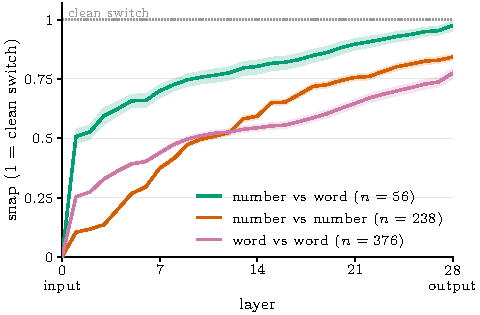
\includegraphics{fig3.pdf}
\end{minipage}\hfill
\begin{minipage}[c]{3.1in}
\caption{Blends collapse gradually through the layers.
At each fork we feed a blend of the chosen token and the runner-up and measure how sharply each layer
resolves it (snap: 0 = carried linearly, 1 = clean switch).
Snap is 0 at the input by construction and reaches 0.98 (number vs word), 0.84 (number vs number) % C21.4
and 0.77 (word vs word) at the output. % C21.4
Number vs word snaps hardest at every layer from 1 to 28; number vs number starts slowest % C21.24
and passes word vs word at layer 13. % C21.23
Bands: 95\% bootstrap CIs over problems.
670 unique forks from 40 GSM8K problems (items 10--49). % C21.1 C21.3
Inputs are sweeps between two candidates at forks, not the lopsided blends real runs feed (\cref{sec:q3}).}
\label{fig:snap}
\end{minipage}
\end{figure}

\Cref{fig:snap} shows the result for the 670 unique forks of Exp~21. % C21.1
Snap rises from 0 at the input to between 0.37 and 0.70 at layer 7, % C21.4
and to between 0.77 and 0.98 at the output. % C21.4
How far the two candidates differ in kind matters at the output.
Number vs word snaps hardest (0.98, 95\% CI [0.95, 1.00]), % C21.4 C21.5
then number vs number (0.84 [0.83, 0.86]) % C21.4 C21.5
and word vs word (0.77 [0.75, 0.79]). % C21.4 C21.5
This order holds at the output, not at every layer.
Number vs word is highest at every layer from 1 to 28, % C21.24
but number vs number starts slowest: it is below word vs word at layers 1 to 12 % C21.23
and above it from layer 13 to the output. % C21.23
At an exact 50/50 input, the next token is the pure chosen token's or the pure runner-up's % C21.6
at 95\% (number vs number), 98\% (number vs word) and 88\% (word vs word) of the forks where the two differ. % C21.6
The blended states also stay close to the line between the two pure states:
for number vs number at the output, the distance off the line is 0.28 of the distance between them. % C21.13
The noise that produced the trace does not change how a blend is processed
(number vs number at the output: 0.85 for forks from vanilla traces, 0.84 from Gumbel traces). % C21.14
Both pre-registered predictions on collapse were met (P1, P2; \cref{app:prereg}).

\paragraph{Answer.}
Only partly.
By the output a 50/50 blend is mostly resolved, and the next token follows one of the two candidates
at 88 to 98\% of forks. % C21.6
The collapse is gradual, though: at layer 7 the blend is still far from a clean switch. % C21.4
Whether the runner-up is lost or only absent from the next-token prediction is the next question.

%-------------------------------------------------------------------------------------------------
\subsection{Q2: Is the runner-up stored, and can later text read it back?}\label{sec:q2}

The next-token prediction is not the only place a candidate can survive.
Later steps attend to the keys and values (K,V) of the fork position, so the runner-up could be kept there.
We test this at the forks where the model followed the chosen token at the 50/50 input:
96 number vs number forks from 35 problems and 139 word vs word forks from 40 problems, % C21.28
plus 34 number vs word forks. % C21.7-8

\paragraph{Readback.}
For each fork we build two caches: one with the 50/50 blend of the chosen token and the runner-up at the fork
position, and a control cache with a 50/50 blend of the chosen token and a control token.
The control token is the third-ranked pre-noise candidate, so it also fits the context but holds no runner-up.
We then force a 64-token continuation into both caches. % C21.26
It is either the runner-up's own continuation, or the model's own continuation of the chosen token.
At each forced position we take the model's next-token distribution $p$ at the sampling temperature and place it
on the line from the distribution $p_B$ after the pure runner-up to the distribution $p_A$ after the pure chosen token:
$c = (p - p_B)\cdot(p_A - p_B) / \lVert p_A - p_B\rVert^2$. % SETUP
A score of 1 means ``as if the chosen token had been written'' and 0 ``as if the runner-up had been written''.
The runner-up readback is the control score minus the blend score.
It is above 0 when the blend cache makes the model read the text more as if it had written the runner-up.
Positions where $p_A$ and $p_B$ differ by less than 0.05 in total variation are skipped. % SETUP

\begin{figure}[t]
\centering
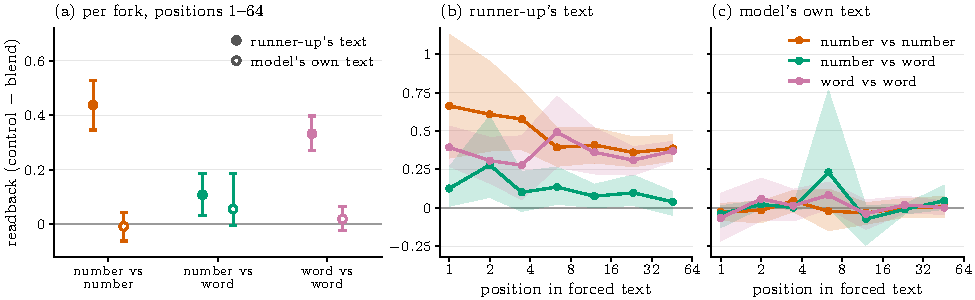
\includegraphics{fig4.pdf}
\caption{The runner-up is stored and can be read back, but stays dormant on the model's own path.
At forks where the model followed the chosen token, we force a 64-token continuation into the cache built from % C21.26
the 50/50 blend and into a control cache (chosen token blended 50/50 with the third-ranked candidate), and score the next-token
predictions from 0 (as if the runner-up had been written) to 1 (as if the chosen token had).
Readback = control minus blend; above 0 means the runner-up is read back from the cache.
(a) Per fork: with the runner-up's text, +0.44 (number vs number), +0.11 (number vs word) % C21.7-8
and +0.33 (word vs word); % C21.7-8
with the model's own text, $-0.01$ to $+0.06$, with every CI including 0. % C21.9 C21.25
(b) With the runner-up's text, the readback stays above 0 in every position bin up to 64 tokens % C21.26
for number vs number and word vs word.
(c) With the model's own text, the CI includes 0 in every bin for number vs number and word vs word. % C21.27
Positions are binned on a log scale; \cref{fig:readback-unbinned} shows them unbinned.
Bars and bands: 95\% bootstrap CIs over problems.
$n$ = 96, 34 and 139 forks. % C21.7-8
Exact 50/50 blends are the most favourable case for the runner-up, so these values are likely an upper bound for real forks,
if readback grows with the residual (\cref{sec:q3}).}
\label{fig:readback}
\end{figure}

With the runner-up's text, the blend cache reads it back (\cref{fig:readback}a).
The readback is $+0.44$ for number vs number (95\% CI [0.35, 0.53]), % C21.7-8
$+0.33$ for word vs word ([0.27, 0.40]) % C21.7-8
and $+0.11$ for number vs word ([0.03, 0.19]). % C21.7-8
The stored runner-up moves the model 0.44 of the way, % C21.7-8
on number vs number forks, toward reading the text as if it had written the runner-up itself.
For number vs word the runner-up is mostly erased, but not completely.
The effect lasts: for number vs number and word vs word the CI stays above 0 in every position bin up to 64 tokens % C21.26
(\cref{fig:readback}b), and without binning the mean is above 0 at every single position from 1 to 16 % C21.38
(\cref{fig:readback-unbinned}).
With the model's own text the picture is different (\cref{fig:readback}c).
The readback is $-0.01$ [$-0.06$, 0.04] for number vs number, % C21.9 C21.25
$+0.02$ [$-0.02$, 0.07] for word vs word % C21.9 C21.25
and $+0.06$ [$-0.00$, 0.19] for number vs word, % C21.9 C21.25
and the CI includes 0 in every position bin for number vs number and word vs word. % C21.27
On the path the model actually takes, the runner-up is dormant.
These results met pre-registered predictions P3 and P4 (\cref{app:prereg}).

\paragraph{Where the runner-up is stored.}
To locate it, we swap only the fork position's keys and values between the blend cache and the control cache,
at one layer or one block of layers, and force the runner-up's text as before.
\emph{Remove} puts the control's K,V into the blend cache and asks whether these layers are needed.
\emph{Insert} puts the blend's K,V into the control cache and asks whether they are enough.
We report the pooled share of the blend--control readback gap that the swap closes, summed over forks.

\begin{figure}[t]
\centering
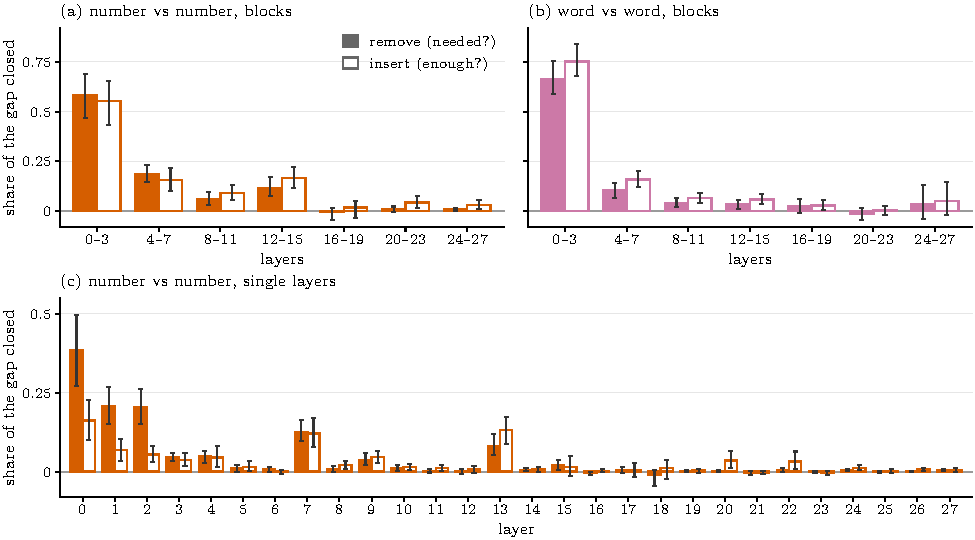
\includegraphics{fig5.pdf}
\caption{The runner-up is stored mostly in the early layers.
At each fork (50/50 blend; forks where the model followed the chosen token) we swap the keys and values of the
fork position between the blend cache and the control cache at a set of layers, and report the pooled share of
the blend--control readback gap this closes (summed over forks).
Remove (filled): put control K,V into the blend cache (are these layers needed?).
Insert (open): put blend K,V into the control cache (are they enough?).
(a, b) Layers 0--7 close 0.77 / 0.71 (number vs number, remove / insert) % C21.10
and 0.77 / 0.91 (word vs word) of the gap; % C21.10
layers 12--27 close 0.12 / 0.26 and 0.08 / 0.14. % C21.11
(c) Number vs number, single layers: the early effect sits in layers 0--2 % C21.19 C21.29
(remove 0.38, 0.21, 0.20). % C21.19 C21.29
Outside layers 0--3, only layers 7 (0.13 / 0.12) and 13 (0.08 / 0.13) stand out, with CIs excluding 0; % C21.19 C21.20 C21.30
every other layer closes at most 0.05. % C21.30
Note the different $y$-axis in (c).
The single-layer analysis was not pre-registered; \cref{tab:fig5-singles} shows these layers survive a
Bonferroni correction over all 56 single-layer tests. % C21.35
\Cref{tab:fig5-robust} shows the shares hold when any one problem, or forks with a small gap, are dropped;
\cref{fig:perfork} shows the per-fork spread, which is wide for layer 0.
Error bars: 95\% bootstrap CIs over problems.
96 forks from 35 problems (number vs number) and 139 forks from 40 problems (word vs word). % C21.28
Number vs word is not shown: its gap ($+0.11$) is too small to localise (\cref{tab:fig5-nw}). % C21.7-8
All shares are measured at exact 50/50 blends, the most favourable case for the runner-up, so these shares are likely an upper bound for real forks.}
\label{fig:patch}
\end{figure}

The runner-up is held mostly in layers 0 to 7 (\cref{fig:patch}a,b). % C21.10
These layers close a pooled share of 0.77 (remove) and 0.71 (insert) of the gap for number vs number, % C21.10
and 0.77 and 0.91 for word vs word. % C21.10
Layers 12 to 27 close 0.12 and 0.26, and 0.08 and 0.14. % C21.11
This split was pre-registered (P5, P6; the smallest lower bound of the difference is 0.31). % C21.22
By blocks of four layers, layers 0--3 carry most of it % C21.15 C21.17
(number vs number 0.58 / 0.55, word vs word 0.66 / 0.75 for remove / insert), % C21.15 C21.17
layers 4--7 add 0.19 / 0.16 and 0.10 / 0.16, % C21.15 C21.17
and every block from layer 16 on closes at most 0.04 for number vs number. % C21.16
For word vs word every block from layer 8 on closes at most 0.07. % C21.18
Across blocks the effects add up: the number vs number blocks sum to 0.95 (remove) and 1.06 (insert). % C21.21

Two findings below this level are exploratory: we found them after looking at the data.
First, for number vs number the early effect sits in layers 0 to 2 (\cref{fig:patch}c). % C21.29
Single layers close 0.38 / 0.16 (layer 0), 0.21 / 0.07 (layer 1) and 0.20 / 0.05 (layer 2). % C21.19 C21.29
Outside layers 0--3 only layers 7 (0.13 / 0.12) and 13 (0.08 / 0.13) stand out; % C21.19 C21.30
every other layer closes at most 0.05. % C21.30
All five survive a Bonferroni correction over the 56 single-layer tests, % C21.35
although the insert effects of layers 1 and 2 only just do (corrected lower bound 0.01; \cref{tab:fig5-singles}). % C21.35
Second, inside layers 0--3 single layers do not add up to their block. % C21.31
Removing one layer at a time sums to 0.84 against 0.58 for the block, % C21.31
and inserting one at a time sums to 0.32 against 0.55. % C21.31
One reading is that the runner-up is held redundantly across layers 0--2: % C21.29
removing any one of them breaks the readback, but no single one carries it.
Another is that the readback score saturates, since it is a projection that can pass 1.
Our data do not separate the two.

The pooled shares are not driven by one problem or a few forks.
Dropping any one problem changes a pooled share by at most 0.04, % C21.33
and keeping only forks with a gap of at least 0.1 changes none by more than 0.03 (\cref{tab:fig5-robust}). % C21.40
The 10 forks with the largest gap carry 0.27 (number vs number) and 0.24 (word vs word) of the total gap. % C21.37
Layer 0 is the exception to a uniform picture (\cref{fig:perfork}).
Its pooled remove share is 0.38, but the median fork's share is 0.12 % C21.34
(insert: 0.16 against 0.02), with quartiles of 0.01, 0.12 and 0.68. % C21.34 C21.39
Layer 0 matters a lot at some forks and little at about half of them.

Part of the early-layer share is expected by construction.
At layer 0 the keys and values of the fork position depend only on the fed embedding, which contains the runner-up,
so the runner-up is present there as an echo of the input.
There is also a small processed trace: for number vs number, layers 7 and 13 stand out (exploratory, as above). % C21.19

\paragraph{Answer.}
Yes.
The runner-up is stored, mostly in the keys and values of layers 0 to 7 and partly as an echo of the input, % C21.10
and text that turns toward it reads it back for the whole 64-token continuation. % C21.26
On the model's own path it stays dormant.
All of this is measured at exact 50/50 blends, the most favourable case for the runner-up.

%-------------------------------------------------------------------------------------------------
\subsection{Q3: What blends does the noise actually feed?}\label{sec:q3}

\Cref{sec:q1,sec:q2} feed exact 50/50 blends.
Real runs feed whatever blend the noise produces, so we record it.
Exp~22 replays ordinary vanilla, Gumbel and Dirichlet runs on 20 problems and logs the pre-noise and the fed weights % C22.7
at every thinking step.
Forks make up 9.2\% (vanilla), 13.0\% (Gumbel) and 13.3\% (Dirichlet) of thinking steps. % C22.1 C22.2 C22.3
There are 3,774, 5,761 and 4,978 forks; each arm is its own run, so the forks differ. % C22.7

\paragraph{The top token of \GST{} is a sampled token.}
Gumbel noise makes the top token of the fed blend a sample from the filtered distribution.
This is the Gumbel-max trick \citep{gumbel1954statistical,maddison2014sampling}:
the token with the largest perturbed log-probability is distributed exactly as a draw from the distribution, and the
softmax at temperature $\tau$ does not change which token is largest.
\citet{wu2025single} cite the trick to motivate Gumbel-Softmax; we check its consequence in the logged runs.
At forks, Gumbel makes a token other than the pre-noise top token the winner at a rate of 0.45, % C22.4
and ordinary sampling would do so at 0.45 (one minus the pre-noise top weight). % C22.4
The difference is 0.00 (95\% CI [$-0.01$, 0.02]). % C22.8
Binned by the sampling rate, Gumbel stays within 0.04 of sampling in every bin with at least 100 forks % C22.9
(\cref{fig:fed}b).
Dirichlet noise has no such guarantee, and it does not match sampling:
it flips less often, by $-0.03$ [$-0.04$, $-0.02$], and is below sampling in all 10 bins. % C22.8 C22.10
Its winner leans toward the pre-noise top token.
So Dirichlet \ST{} is not sampling in disguise in the exact sense that \GST{} is.

\begin{figure}[t]
\centering
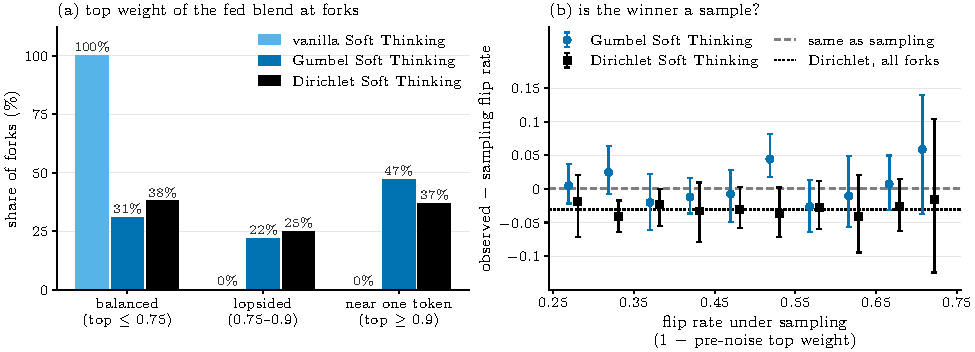
\includegraphics{fig6.pdf}
\caption{Noise turns real forks into lopsided blends, and Gumbel's winner is a sample.
A fork is a thinking step where the pre-noise runner-up holds at least 25\% of the weight % SETUP
(9.2\% of steps for vanilla, 13.0\% for Gumbel, 13.3\% for Dirichlet). % C22.1 C22.2 C22.3
(a) Share of forks by the top weight of the blend actually fed.
Vanilla feeds the pre-noise weights unchanged, so it shows what the model wanted: every fork is balanced % C22.5 C22.11
(top weight at most 0.75, by the fork rule). % C22.11
Gumbel feeds a near one-token blend (top weight at least 0.9) at 47\% of forks and Dirichlet at 37\%. % C22.11
The median fed blend has a residual (weight off the top token) of 0.12 for Gumbel and 0.17 for Dirichlet, % C22.12
against 0.44 before noise. % C22.12
(b) How often noise makes a token other than the pre-noise top one the winner, minus how often ordinary sampling
would (1 minus the pre-noise top weight), with forks binned by the sampling rate.
Gumbel matches sampling: 0.00 [$-0.01$, 0.02] overall and within 0.04 in every bin with at least 100 forks. % C22.8 C22.9
Dirichlet flips less often than sampling in every bin, $-0.03$ [$-0.04$, $-0.02$] overall (dashed line). % C22.8 C22.10
Vanilla never flips (not shown). % C22.1
Error bars: 95\% bootstrap CIs over problems.
3,774 (vanilla), 5,761 (Gumbel) and 4,978 (Dirichlet) forks from 20 GSM8K problems; % C22.7
each arm is its own run, so the forks differ.}
\label{fig:fed}
\end{figure}

\paragraph{The residual is real but small.}
Before noise, the median fork has a residual of 0.44: the model splits its weight. % C22.12
Vanilla feeds these weights unchanged, so every vanilla fork is balanced, % C22.5 C22.11
with a top weight of at most 0.75 by the fork rule (\cref{fig:fed}a). % C22.11
Noise makes the fed blends lopsided.
\GST{} feeds a blend near one token (top weight at least 0.9) at 47\% of forks, % C22.2 C22.11
a lopsided blend (0.75 to 0.9) at 22\% and a balanced one at 31\%. % C22.11
The median fed blend has a top weight of 0.88 and a residual of 0.12. % C22.2 C22.12
Dirichlet gives 37\%, 25\% and 38\%, with a median residual of 0.17. % C22.11 C22.12
At the median fork, almost all of the residual sits on one other token % C22.12
(0.99 of it for Gumbel and 1.00 for Dirichlet). % C22.12
Over all thinking steps, the fed blend is near one token at 85\% (Gumbel) % C22.2
and 83\% (Dirichlet) of steps. % C22.3
We had pre-registered that Gumbel would feed near one-token blends at 70\% or more of forks and 90\% or more % PR(Exp 22 P1, Exp 22 P3)
of steps; both failed (\cref{app:prereg}).

\paragraph{Answer.}
\GST{} feeds the sampled token plus a residual.
At forks the residual is real but small: its median is 0.12, % C22.12
and at about half of forks the blend is near one token. % C22.11
The exact 50/50 blends of \cref{sec:q1,sec:q2} are the extreme case, so the storage and readback measured there are
likely an upper bound on what a real fork carries, if readback grows with the residual.

%-------------------------------------------------------------------------------------------------
\subsection{Q4: Does the model use the residual?}\label{sec:q4}

If the top token of \GST{} is a sampled token, any difference from sampling must come from the residual.
Exp~23 isolates it.
Three arms run in lockstep on 100 GSM8K problems never used before (items 50--149), % C23.1
with shared Gumbel noise keyed by seed, step and token id.
\emph{Sampling} feeds the top token alone (a one-hot input).
\emph{\ST{}} feeds the full Gumbel blend.
The \emph{\ctrl{}} keeps the top token at its blend weight and moves the residual onto a random vocabulary token.
Because the noise is shared, the three arms pick the same top token at a step until their contexts differ,
and they differ only in where the residual goes.
The random rows have the same median norm as all real-token rows, and 0.994 of that of reasoning tokens (\cref{app:norms}), % C23.10 C23.11
so the control carries a residual of the same size and a typical norm.

\begin{table*}[t]
\centering
\small
\caption{Neither Gumbel Soft Thinking nor the random-residual control differs detectably from sampling in accuracy, and the paired intervals still allow differences of several points either way. Accuracy comparison: sampling and Gumbel Soft Thinking at seeds 0 and 1 on the same 30 problems, so their 60 runs are clustered by problem and their CIs are 95\% bootstrap intervals over problems (per seed: sampling 27 and 25 of 30, Gumbel 26 and 26); vanilla Soft Thinking has one seed and a Wilson interval. Its difference from sampling is paired on seed 0 (Newcombe interval); Gumbel's is the mean per-problem difference over both seeds, bootstrapped over problems. McNemar uses the seed 0 runs, the only seed vanilla has. Vanilla hit Cold Stop on 14 of 30 runs, and all 5 runs without an answer ended there; against Gumbel (seed 0) it is 1 vs 5, $p = 0.22$. Coupled ablation: seed 0; the three arms share their noise, and the random-residual control moves the residual to a random token. Accuracy has Wilson intervals and the paired difference a Newcombe hybrid-score interval. Its problems are not used in any other experiment. McNemar: exact two-sided test on the problems where exactly one of the pair is correct.}
\label{tab:accuracy}
\begin{tabular}{@{}lrrccccc@{}}
\toprule
 & & & & & \multicolumn{3}{c}{McNemar vs sampling} \\
\cmidrule(lr){6-8}
Arm & Runs & Correct & Accuracy [95\% CI] & Difference vs sampling [95\% CI] & Arm only & Sampling only & $p$ \\
\midrule
\multicolumn{8}{@{}l}{\emph{Accuracy comparison: GSM8K items 0--29}} \\
Sampling & 60 & 52 & 0.87 [0.75, 0.97] &  &  &  &  \\
Vanilla Soft Thinking & 30 & 22 & 0.73 [0.56, 0.86] & $-$0.17 [$-$0.33, $-$0.01] & 0 & 5 & 0.06 \\
Gumbel Soft Thinking & 60 & 52 & 0.87 [0.73, 0.97] & 0.00 [$-$0.10, +0.10] & 1 & 2 & 1.00 \\
\addlinespace
\multicolumn{8}{@{}l}{\emph{Coupled ablation: GSM8K items 50--149, arms in lockstep}} \\
Sampling & 100 & 86 & 0.86 [0.78, 0.91] &  &  &  &  \\
Gumbel Soft Thinking & 100 & 88 & 0.88 [0.80, 0.93] & +0.02 [$-$0.05, +0.09] & 6 & 4 & 0.75 \\
Random-residual control & 100 & 82 & 0.82 [0.73, 0.88] & $-$0.04 [$-$0.11, +0.03] & 3 & 7 & 0.34 \\
\bottomrule
\end{tabular}
\end{table*}


\begin{figure}[t]
\centering
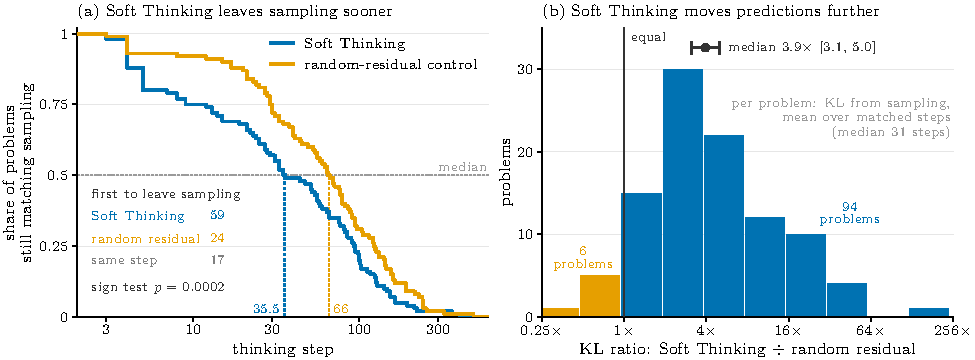
\includegraphics{fig7.pdf}
\caption{The model reads the residual.
Three arms run in lockstep with shared noise on 100 GSM8K problems: % C23.1
sampling (top token only), \ST{} (full blend) and a \ctrl{} (the residual moved to a random token).
(a) Share of problems on which each arm has so far picked the same token as sampling at every thinking step.
\ST{} leaves sampling sooner: median step 35.5 vs 66; % C23.4
it leaves first on 59 problems, the random residual on 24, both at once on 17 (sign test $p = 0.0002$). % C23.5-6
(b) Per problem, how far \ST{} moves next-token predictions away from sampling's, divided by how far the
random residual does (KL divergence, averaged over the steps before either arm leaves sampling;
median 31 steps). % C23.15
\ST{} moves them more on 94 of 100 problems; % C23.8
the median problem is 3.9 times (marker: median and 95\% bootstrap CI over problems, [3.1, 5.0]). % C23.15
Items 50--149, not used in any other experiment; seed 0.} % C23.1
\label{fig:ablation}
\end{figure}

\paragraph{The model reads the residual.}
\ST{} leaves sampling sooner than the \ctrl{} (\cref{fig:ablation}a).
The first step at which its token differs from sampling's has a median of 35.5, against 66 for the control. % C23.4
Paired by problem, \ST{} leaves first on 59 problems, the control on 24, and both at the same step on 17 % C23.5-6
(sign test, $p = 0.0002$). % C23.5-6
To compare the arms before their texts differ, we average the KL divergence of each arm's next-token
distribution from sampling's over the steps before either arm leaves sampling
(a median of 31 steps per problem). % C23.15
\ST{} moves the predictions more than the control on 94 of 100 problems. % C23.8
The median per-problem ratio is 3.9 (95\% CI [3.1, 5.0]; \cref{fig:ablation}b). % C23.15
We chose the median after seeing that the ratio of the means, 5.7, is driven by a few problems: % C23.14
five problems hold 0.54 of \ST{}'s total, and without them the ratio of means is 3.1. % C23.14
The pre-registered prediction E1 expected the opposite direction, that the residual would move predictions less than
a random one (\cref{app:prereg}).

\paragraph{Accuracy does not change detectably.}
\Cref{tab:accuracy} compares accuracy.
In Exp~23, \ST{} solves 88 of 100 problems and sampling 86. % C23.1
The discordant pairs split 6 to 4 (McNemar $p = 0.754$), % C23.2
and the two arms reach the same final answer on 84 problems. % C23.2
The \ctrl{} solves 82 (3 to 7 against sampling, $p = 0.344$), % C23.1 C23.3
and it also reaches sampling's final answer on 84 problems. % C23.3
So the real residual changes the final answer no more often than a random one.
In Exp~16, on different problems (items 0--29), \GST{} and sampling both solve 52 of 60 runs; % C16.1 C16.3
on seed 0, \GST{} alone is right on 1 problem and sampling alone on 2 ($p = 1.00$). % C16.12
Vanilla \ST{} shows the Greedy Pitfall of \citet{wu2025single} in its behaviour:
14 of its 30 runs end in Cold Stop, a repetition loop, % C16.2
and all of its 5 runs without an answer are among them. % C16.2 C16.8
\GST{} never hits Cold Stop, % C16.3
and sampling and \GST{} solve 4 of those 5 problems in every run. % C16.9
Vanilla's accuracy (22 of 30) is lower, but the difference is not significant at this size % C16.2
($p = 0.062$ against sampling, $p = 0.22$ against Gumbel). % C16.13 C16.5
These tests are small.
With only 6 and 4 discordant problems in Exp~23, an effect of a few points in either direction cannot be excluded. % C23.2
The pre-registered prediction E2 (no detectable accuracy difference, judged on the point estimate) was met.

\paragraph{Answer.}
The model reads the residual: it moves next-token predictions a median 3.9 times as much as a random residual of the % C23.15
same size, and it makes \ST{} leave sampling sooner.
Yet accuracy does not change detectably, and the real residual changes final answers no more often than a random one.
The residual is read but, within the power of our test, not used.

\section{Discussion}\label{sec:discussion}

\paragraph{Reconciling with Wu et al.~\cite{wu2025single}.}
Wu et al.~\cite{wu2025single} report that \GST{} outperforms matched sampling, with the same temperature, top-$p$ and top-$k$,
on three 32B reasoning models. % CITE(wu2025single)
The gain, averaged over their eight benchmarks, is $+0.42$ to $+1.05$ points, with no variance or significance % CITE(wu2025single)
reported; GPQA-Diamond shows the largest gains, up to $+5.05$ points (their Table~2). % CITE(wu2025single)
At 1.5B on GSM8K we find no detectable difference % SETUP
(accuracy comparison: 52 of 60 for both; coupled ablation: 88 vs 86 of 100, McNemar $p = 0.754$). % C16.1 C16.3 C23.1 C23.2
The two findings are compatible.
Wu et al.\ motivate Gumbel-Softmax through the Gumbel-max trick; its consequence is that the top token of \GST{} is
distributed exactly as a sampled token, which we confirm (flip rate 0.45 for both). % C22.4
Dirichlet noise has no such guarantee, and in our runs its top token flips 0.03 less often than a sampled token % C22.8
would.
Wu et al.\ also find Dirichlet no better than sampling, although our Dirichlet uses $\gamma = 1.0$ % SETUP
and theirs 4.0 by default. % CITE(wu2025single)
Any accuracy difference between \GST{} and sampling must therefore come from the residual.
Our coupled ablation holds the noise fixed and removes only the residual.
The model reads it, yet accuracy does not change detectably.
Our paired interval runs from 5 points below sampling to 9 points above it, a range that includes the gains % C23.17
Wu et al.\ report.
For the Gumbel variant this refines their single-threaded account: the top token is a sample, and the residual is
read but leaves accuracy unchanged within our power.
Three differences could separate the settings.
A 32B model may use a residual that % CITE(wu2025single)
a 1.5B model only stores. % SETUP
GSM8K is near ceiling for our model (86 to 88\% in the coupled ablation), while the largest reported gains are on harder % C23.1
benchmarks.
Our study lacks the power to resolve effects of a few points, and Wu et al.\ report no variance.
Running the coupled ablation on a 32B model and a harder benchmark would show which explanation applies. % CITE(wu2025single)

\paragraph{The tension with Rizvi-Martel et al.~\cite{rizvimartel2026illusion}.}
They conclude that off-the-shelf models collapse \ST{} inputs within the first few layers, while our
\cref{fig:snap} shows a gradual collapse that is complete only at the output.
The two results measure different things.
Their evidence for early collapse comes from vanilla \ST{}, every 50 decoding steps: the logit-lens entropy of % CITE(rizvimartel2026illusion)
separate soft and discrete runs, and the KL divergence between forward passes with the soft input and with its top
token.
Those inputs are close to one token on average (mean mixing-weight entropy 0.10 to 0.18 nats), so little blend is % CITE(rizvimartel2026illusion)
left to lose.
We condition on forks, feed exact 50/50 blends of the two candidates, and track the position between them at every
layer.
On these inputs the blend is still far from a clean switch at layer 7 (snap 0.37 to 0.70). % C21.4
This agrees with their own test on uniform mixtures, where entropy drops only at the last layers, and with
Backour~\cite{backour2026dynamics}, who finds that Qwen models accumulate collapse toward the output.
Collapse in the next-token readout also does not mean the runner-up is lost: a trace of it persists, mostly in the
keys and values of layers 0 to 7, and shifts later predictions toward it (\cref{sec:q2}). % C21.10
Our blends are 50/50, likely an upper bound on real forks, where the median residual is 0.12. % C22.12

\paragraph{What our evidence says about superposition.}
Our results separate three levels of token-level superposition: a second candidate present in the input, read by
the model, and used.
The forced 50/50 blends are present in the input, and a trace of the runner-up persists in the cache.
The residual of \GST{} is read: it shifts next-token predictions far more than a random residual.
We find no evidence that it is used.
For that, the trace would have to shift predictions on the model's own path, where we detect no shift, and the
residual would have to change answers, where we detect no accuracy change and the real residual changes answers
no more often than a random one.
Two limits keep this from being a general verdict on superposition.
Our blends are forced, not learned; models trained with latent thoughts from scratch show signs of using
superposition \cite{rizvimartel2026illusion}, and reinforcement learning with soft tokens is now practical
\cite{butt2025soft,zheng2025softgrpo}.
And we test single positions, not whole reasoning paths: a model could in principle keep two lines of reasoning
alive across many steps without either one leaving a detectable trace at a single fork.
The coupled ablation applies to trained models unchanged: shared noise gives the arms the same top token until their
contexts diverge, so the residual is the only source of divergence.

\section{Limitations}\label{sec:limitations}

We study one model, DeepSeek-R1-Distill-Qwen-1.5B, on one task, GSM8K, mostly with one seed. % SETUP
Larger models or harder tasks may use the residual where this model does not.
Accuracy on GSM8K is near ceiling for this model, which leaves little room for the residual to help.
The accuracy tests have low power: the coupled ablation has only 6 and 4 discordant problems, and its paired % C23.2
interval allows differences from 5 points below sampling to 9 points above, so our null result is an absence of % C23.17
evidence at this size.
Our tests are at the level of single token positions.
We do not test whether the model carries whole reasoning paths in superposition across many steps, and every blend
we study is a forced superposition built at the input, not a learned one \cite{rizvimartel2026illusion}.
The cache results (\cref{sec:q1,sec:q2}) use exact 50/50 blends at forks where the model followed the chosen
token, the most favourable case for the runner-up.
Real Gumbel forks feed a median residual of 0.12, so these results are likely an upper bound on what real runs carry, % C22.12
if readback grows with the residual; we did not measure readback at realistic weights.
The readback and snap scores are projections onto the line between two pure states, so they can saturate or pass 1;
this is one of two readings of the non-additivity inside layers 0--3. % C21.31
The single-layer patching results are exploratory and were found after looking at the data.
The experiments are not independent samples of problems: the fed-blend log uses a subset of the fork probe's
problems and overlaps the accuracy comparison.
Our Dirichlet noise uses $\gamma = 1.0$, % SETUP
while Wu et al.~\cite{wu2025single} use 4.0 by default, so our Dirichlet result may not transfer to their setting. % CITE(wu2025single)
Finally, our decoding settings differ from those of Wu et al.~\cite{wu2025single} (top-$k$, thinking budget, Cold Stop); they
are matched across our own arms, but our absolute accuracies are not comparable with theirs.

\section{Conclusion}\label{sec:conclusion}

\GST{} feeds a sampled token plus a residual.
In a 1.5B reasoning model on GSM8K, the model stores the runner-up, mostly in early-layer keys and values, and reads the % SETUP
residual, but accuracy does not change detectably.
In accuracy \GST{} at this scale behaves like sampling, although internally the residual is not ignored.
Testing larger and trained models with the same coupled ablation is the clearest next step.


\bibliographystyle{IEEEtran}
\bibliography{refs}

\appendix
\section{Pre-registration record}\label{app:prereg}

We committed predictions with numeric thresholds to our git repository before each run.
Git dates are set by the local machine, so they show the order of commits, not an external timestamp; the Kaggle
notebook version times give a second record.
\Cref{tab:prereg} lists every prediction as written and its outcome, including the ones that failed.

\textbf{Fork probe} (P1--P6) was committed on 7 October 2026 (commit \texttt{7d41cd4}), before any of its results. % SETUP
The thresholds were set on a 10-item pilot (items 0--9) and tested on 40 held-out items (10--49). % SETUP
The pilot's raw outputs were not saved, so we report no pilot numbers.
P1 was written as ``snap $\geq 0.6$'' before we rescaled snap so that a perfect switch scores 1; % PR(P1) SETUP
on the rescaled measure the same threshold is 0.66, and P1 is met on both scales. % PR(P1)

\textbf{Fed-blend log} (P1--P3) and \textbf{coupled ablation} (E1, E2) were committed on 10 October 2026 (commit \texttt{d2e770f}), % SETUP
before either experiment was run.
After writing P1--P3 but before running the fed-blend log, we derived the distribution of the fed top weight in closed form.
It showed that a 50/50 fork gives a fed top weight of at least 0.9 with probability 0.50 under Gumbel noise, and a % C22.6
75/25 fork with probability 0.60, so P1 and P2 could not reach their 70\% thresholds. % C22.6 PR(Exp 22 P1)
We kept P1 and P2 as written and added A1--A3 in the same commit, again before running.

Two predictions failed in an informative way.
Fed-blend log P3 expected near one-token blends at 90\% of all thinking steps; Gumbel reached 85\%. % PR(Exp 22 P3)
E1 expected the residual to move predictions less than a random residual, as it would if the model ignored the
residual; the result went the other way (\cref{sec:q4}).
E1 was written for the KL averaged over each arm's own steps up to and including its first divergence, and the
table reports it on that measure: \ST{} moved predictions less on 14 of 100 problems (mean KL 0.545 against % C23.16
0.009). % C23.16
In the main text we report the KL over steps matched across arms, because the registered measure is dominated by the
divergence step itself; on matched steps \ST{} moved predictions less on 6 of 100. % PR(Exp 23 E1)
The verdict is the same under both measures.
One summary statistic was also chosen after seeing the data: we report the median per-problem KL ratio (3.9) % C23.15
because the ratio of means (5.7) turned out to be driven by five problems (\cref{sec:q4}). % C23.14

\section{Robustness of the storage results}\label{app:robust}

The tables and figures in this appendix back \cref{fig:readback,fig:patch}.
\Cref{tab:fig5-robust} recomputes the pooled patching shares when only forks with a gap of at least 0.1 are kept, % C21.32
when each problem is dropped in turn, and as a median over forks.
\Cref{tab:fig5-singles} gives the number vs number single layers that stand out, with Bonferroni-corrected lower
bounds over all 56 single-layer tests. % C21.35
\Cref{tab:fig5-nw} reports the number vs word blocks, whose gap is too small to localise.
\Cref{fig:readback-unbinned} shows the readback at single positions of the forced text, and \cref{fig:perfork} the
per-fork spread behind the pooled shares.

\begin{table*}[t]
\centering
\small
\caption{Robustness of the patching shares in Fig.~5. Pooled: share of the summed blend--control gap closed (as plotted). Gap $\geq$ 0.1: the same, keeping only forks whose gap is at least 0.1. Leave one out: range of the pooled share when each problem is dropped in turn. Median: median of per-fork shares over forks with gap $\geq$ 0.1. Fork probe, GSM8K items 10--49, 50/50 blends, forks where the model followed the chosen token.}
\label{tab:fig5-robust}
\begin{tabular}{lcccccccc}
\toprule
 & \multicolumn{4}{c}{Remove} & \multicolumn{4}{c}{Insert} \\
\cmidrule(lr){2-5} \cmidrule(lr){6-9}
Patched & Pooled & Gap $\geq$ 0.1 & Leave one out & Median & Pooled & Gap $\geq$ 0.1 & Leave one out & Median \\
\midrule
\multicolumn{9}{l}{\emph{Number vs number: 96 forks, 78 with gap $\geq$ 0.1}} \\
layers 0--3 & 0.58 & 0.56 & 0.56--0.62 & 0.53 & 0.55 & 0.54 & 0.54--0.59 & 0.49 \\
layers 4--7 & 0.19 & 0.19 & 0.18--0.20 & 0.16 & 0.16 & 0.16 & 0.14--0.17 & 0.10 \\
layers 8--11 & 0.06 & 0.06 & 0.05--0.06 & 0.02 & 0.09 & 0.09 & 0.08--0.10 & 0.04 \\
layers 12--15 & 0.12 & 0.10 & 0.11--0.12 & 0.06 & 0.17 & 0.16 & 0.15--0.18 & 0.10 \\
layer 0 & 0.38 & 0.36 & 0.35--0.41 & 0.12 & 0.16 & 0.16 & 0.14--0.17 & 0.02 \\
layer 1 & 0.21 & 0.20 & 0.19--0.22 & 0.14 & 0.07 & 0.07 & 0.06--0.08 & 0.05 \\
layer 2 & 0.20 & 0.19 & 0.19--0.22 & 0.12 & 0.05 & 0.06 & 0.05--0.06 & 0.03 \\
layer 7 & 0.13 & 0.13 & 0.12--0.13 & 0.11 & 0.12 & 0.12 & 0.11--0.13 & 0.06 \\
layer 13 & 0.08 & 0.07 & 0.07--0.09 & 0.04 & 0.13 & 0.12 & 0.12--0.14 & 0.05 \\
\addlinespace
\multicolumn{9}{l}{\emph{Word vs word: 139 forks, 108 with gap $\geq$ 0.1}} \\
layers 0--3 & 0.66 & 0.63 & 0.65--0.69 & 0.66 & 0.75 & 0.72 & 0.73--0.77 & 0.78 \\
layers 4--7 & 0.10 & 0.10 & 0.10--0.11 & 0.09 & 0.16 & 0.16 & 0.15--0.17 & 0.15 \\
layers 8--11 & 0.04 & 0.05 & 0.04--0.04 & 0.03 & 0.07 & 0.07 & 0.06--0.07 & 0.06 \\
layers 12--15 & 0.03 & 0.04 & 0.03--0.04 & 0.02 & 0.06 & 0.06 & 0.05--0.06 & 0.05 \\
\bottomrule
\end{tabular}
\end{table*}

\begin{table}[t]
\centering
\small
\caption{Number vs number single layers that stand out in Figure~5c. 95\% CI: bootstrap over problems (2,000 resamples). Corrected lower: lower bound of the Bonferroni-corrected interval for all 56 single-layer tests (28 layers $\times$ remove/insert; 20,000 resamples). Every bound is above 0. The single-layer analysis was not pre-registered.}
\label{tab:fig5-singles}
\begin{tabular}{lcccccc}
\toprule
 & \multicolumn{3}{c}{Remove} & \multicolumn{3}{c}{Insert} \\
\cmidrule(lr){2-4} \cmidrule(lr){5-7}
Patched & Share & 95\% CI & Corrected lower & Share & 95\% CI & Corrected lower \\
\midrule
layer 0 & 0.38 & [0.27, 0.50] & 0.20 & 0.16 & [0.10, 0.23] & 0.06 \\
layer 1 & 0.21 & [0.15, 0.27] & 0.12 & 0.07 & [0.03, 0.10] & 0.01 \\
layer 2 & 0.20 & [0.15, 0.26] & 0.12 & 0.05 & [0.03, 0.08] & 0.01 \\
layer 7 & 0.13 & [0.10, 0.16] & 0.08 & 0.12 & [0.08, 0.17] & 0.05 \\
layer 13 & 0.08 & [0.05, 0.12] & 0.04 & 0.13 & [0.09, 0.17] & 0.06 \\
\bottomrule
\end{tabular}
\end{table}

\begin{table*}[t]
\centering
\small
\caption{Number vs word forks (34 forks from 21 problems), not shown in Fig.~5. The mean blend--control gap is only 0.11, so the shares are unstable (wide CIs, values above 1 and below 0) and cannot localise the runner-up. 95\% CI: bootstrap over problems.}
\label{tab:fig5-nw}
\begin{tabular}{lcccc}
\toprule
 & \multicolumn{2}{c}{Remove} & \multicolumn{2}{c}{Insert} \\
\cmidrule(lr){2-3} \cmidrule(lr){4-5}
Patched & Share & 95\% CI & Share & 95\% CI \\
\midrule
layers 0--3 & 0.98 & [0.63, 2.31] & 0.90 & [0.67, 1.55] \\
layers 4--7 & 0.11 & [0.02, 0.59] & $-$0.01 & [$-$0.24, 0.11] \\
layers 8--11 & $-$0.01 & [$-$0.10, 0.02] & 0.00 & [$-$0.09, 0.06] \\
layers 12--15 & $-$0.03 & [$-$0.12, 0.01] & $-$0.02 & [$-$0.25, 0.05] \\
layers 16--19 & 0.14 & [0.00, 0.38] & 0.08 & [$-$0.03, 0.21] \\
layers 20--23 & 0.07 & [$-$0.01, 0.20] & $-$0.01 & [$-$0.11, 0.05] \\
layers 24--27 & 0.04 & [$-$0.14, 0.12] & 0.03 & [$-$0.09, 0.10] \\
\bottomrule
\end{tabular}
\end{table*}


\begin{figure}[t]
\centering
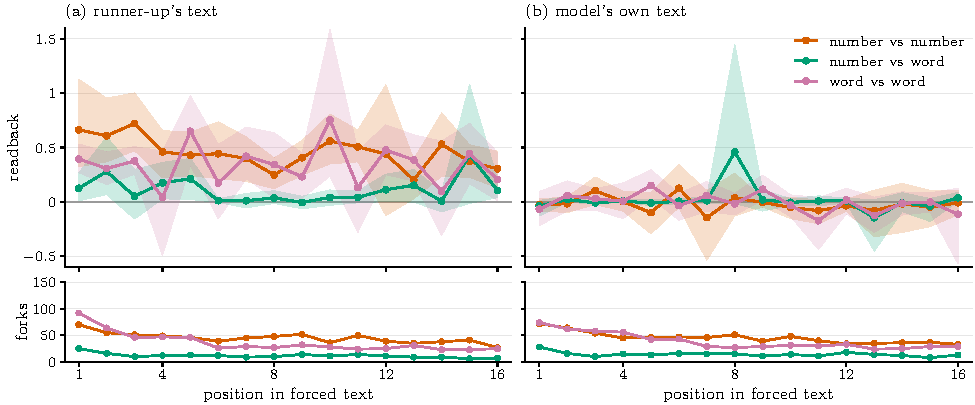
\includegraphics{figA1.pdf}
\caption{Readback at each position of the forced text, without the binning of \cref{fig:readback}b--c.
Top: mean readback (control minus blend) with 95\% bootstrap CIs over problems, for the runner-up's text
(left) and the model's own text (right).
Bottom: number of forks with a defined score at that position (positions where the chosen token and the runner-up
barely differ are skipped).
With the runner-up's text, the mean stays above 0 at every position for number vs number and word vs word; % C21.38
with the model's own text it stays around 0.
Single positions hold few forks, so their CIs are wide; this is why \cref{fig:readback} pools positions into
log-spaced bins.}
\label{fig:readback-unbinned}
\end{figure}

\begin{figure}[t]
\centering
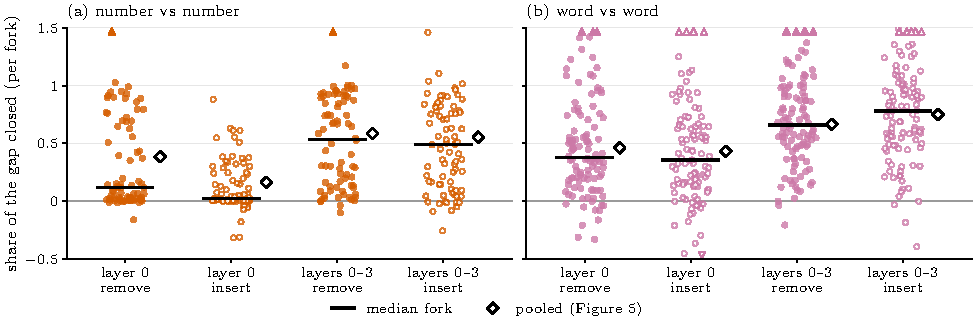
\includegraphics{figA2.pdf}
\caption{Per-fork shares behind the pooled bars of \cref{fig:patch}, for layer 0 and layers 0--3. % C21.31
Each dot is one fork with a blend--control gap of at least 0.1 % C21.32
(78 number vs number forks, 108 word vs word); % C21.32
filled = remove, open = insert.
Black bar: median per fork.
Diamond: pooled share, as plotted in \cref{fig:patch}.
For number vs number, layer 0 is uneven across forks: half of them have a remove
share below 0.12 and a quarter are above 0.68, % C21.39
so the pooled 0.38 sits well above the median fork % C21.34
(0.12; insert: 0.16 vs 0.02). % C21.34
For layers 0--3 the median fork is close to the pooled share. % C21.31
Dots outside the axis range are drawn at its edge as triangles.}
\label{fig:perfork}
\end{figure}

\section{Embedding-norm check for the random-residual control}\label{app:norms}

The \ctrl{} of Exp~23 moves the residual onto a random vocabulary row.
If random rows had much smaller norms than the tokens the model reads while reasoning, the control would carry a weaker
signal than \ST{}, and the KL comparison of \cref{sec:q4} would be unfair to it.
We regenerated the 8,192 random rows that Exp~23 drew, with the same keyed generator, % C23.13
and compared their norms with all real-token rows and with 9,168 tokens from sampled reasoning traces on 5 problems % C23.13
(items 50--54). % C23.10
The median norm is 1.195 for the random rows, 1.195 for all real-token rows, 1.196 when real rows are weighted % C23.10
by usage, and 1.202 for reasoning tokens. % C23.10
The ratio of random rows to reasoning tokens is 0.994 at the median and 0.961 at the mean. % C23.11
The random rows have a heavier low tail (10th percentile 0.897 against 1.058), so a minority of draws carries a % C23.12
weaker signal.
This cannot explain a median KL ratio of 3.9 between \ST{} and the control. % C23.15
These values come from the saved output of a separate GPU run (\texttt{neuralese\_exp23\_norms.py}); the check
scripts compare against that output rather than recompute it from the model.

\section{Reproducibility}\label{app:repro}

\paragraph{Model and software.}
Every experiment loads \url{deepseek-ai/DeepSeek-R1-Distill-Qwen-1.5B} from the Hugging Face Hub at revision
\url{ad9f0ae0864d7fbcd1cd905e3c6c5b069cc8b562}, last modified on 24 February 2025, before any of our runs. % SETUP
The scripts load the Hub identifier, so all runs used this revision.
Each Kaggle notebook installed the latest \texttt{transformers}; the install logs do not print versions, but the
downloaded wheel identifies them.
The fork probe and the coupled ablation used \texttt{transformers} 5.19.0, and the accuracy comparison and the fed-blend log used 5.20.1 (inferred from the wheel size and upload dates). % SETUP
The saved outputs of the accuracy comparison and the fed-blend log come from a later rerun that reproduced the originally logged numbers exactly.
The embedding-norm check (\cref{app:norms}) recorded its full environment: torch 2.11.0+cu128, % SETUP
\texttt{transformers} 5.20.2, CUDA 12.8 and Python 3.13.15 on an NVIDIA Tesla T4. % SETUP
All runs used Python 3.13; torch and CUDA versions are recorded only for the norm check. % SETUP

\paragraph{Code, outputs and checks.}
\Cref{tab:repro} maps each experiment to its script and saved output.
The logs of the Kaggle runs that produced these outputs are in \texttt{kaggle\_logs/}.
Two scripts recompute every number in the paper from the saved outputs and stop on any mismatch:
\texttt{verify\_claims.py} checks the claim ledger, and \texttt{verify\_robustness.py} checks every cell of
\cref{tab:accuracy} and Tables~\ref{tab:fig5-robust}--\ref{tab:fig5-nw}.
A third script, \texttt{paper/check\_numbers.py}, checks that every number in the text matches the ledger row named
next to it in the \LaTeX{} source.
Figures are drawn by one script each (\texttt{figures/make\_*.py}) from the saved outputs.


% AI-use statement. Categories confirmed by the author on 2026-10-26: code for experiments and figures; literature
% summaries. Base text: docs/paper-writing-fixes.md section 5. Generic (venue-neutral) wording for the preprint;
% revise against the chosen venue's policy before submission.
% NOTE FOR THE AUTHOR: this draft's LaTeX text was drafted with an AI assistant from the log, ledger and outline.
% If that stays true of the version you circulate, most venue policies (e.g. ICLR, ACL) expect it to be disclosed.
\section{Use of AI assistants}\label{app:aiuse}

The author used an AI assistant (Anthropic's Claude) to summarise related literature, to draft Python scripts for
the experiments, analyses, figures and tables, and to summarise results and organise experimental data.
The author designed and ran all experiments, reviewed and tested all code, checked every reported number against the
saved outputs and every citation against its source, and takes full responsibility for the content of this paper.


\end{document}
